\documentclass[12pt]{jarticle}
\usepackage[dvipdfmx]{graphicx}
\usepackage[top=25truemm, bottom=25truemm, left=20truemm, right=20truemm]{geometry}
\usepackage{multirow}

\title{IVL2-7/5 データシート}
\author{訳: koktoh (@KokToH\_kuro)}
\date{}

\begin{document}

\maketitle

\section*{まえがき}

これは, http://loststeak.com/ivl2-75-vfd-datasheets/ を意訳したものです.これを使用したことによる事故や損傷については責任を負いかねますので,自己責任の下ご利用ください.

\section{概要}

真空発光多桁インジケータ IVL2-7/5 は,直熱型陰極を持つフラットな三極真空管で,正確な時間を表示するために使用することを目的としており,マルチプレックス駆動で制御することができます.一般的には,車載の時計に使われます.

\section{ピン配置}

    
\begin{minipage}{0.6\linewidth}
    \centering
    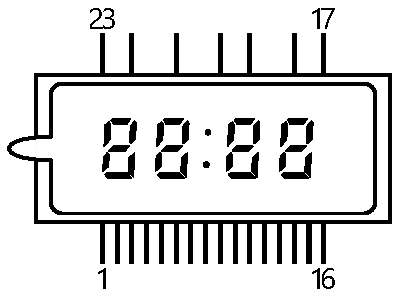
\includegraphics[width=\linewidth]{../img/IVL275.pdf}
\end{minipage}
\hfill
\begin{minipage}[b]{0.35\linewidth}
    \begin{tabular}{rr}
        セグメント高さ & \(10\pm0.05\)  mm \\
        セグメント幅   & \(5.8\pm0.05\) mm
    \end{tabular}
\end{minipage}

\clearpage

\section{各ピン概要}

\begin{figure}[h]
    \begin{minipage}{0.65\linewidth}
        \centering
        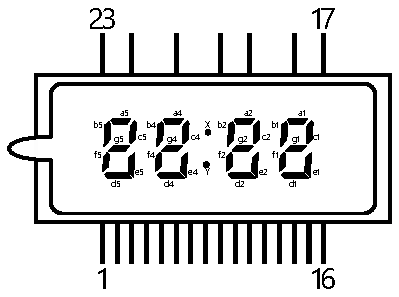
\includegraphics[width=\linewidth]{../img/IVL275_mark_EN.pdf}
    \end{minipage}
    \hfill
    \begin{minipage}{0.2\linewidth}
        \centering
        
\includegraphics[width=\linewidth]{../img/Segment_EN.pdf}
    \end{minipage}
\end{figure}

\begin{table}[h]
    \centering
    \begin{tabular}{|c|l||r|} \hline
        ピン番号 & \multicolumn{1}{c||}{概要} & 定格電圧 \\ \hline \hline
        1, 23 & カソード(フィラメント).真空管内面の導電層. & 2.4V \\ \hline
        2, 22 & 5桁目のセグメントのグリッド. & \multirow{14}{*}{24V} \\ \cline{1-2}
        3 & 3桁目のドットの上側 X のアノード. & \\ \cline{1-2}
        4 & 1, 2, 4, 5桁目のセグメントの g (g1, g2, g4, g5) のアノード. & \\ \cline{1-2}
        5 & 1, 2, 4, 5桁目のセグメントの f (f1, f2, f4, f5) のアノード. & \\ \cline{1-2}
        6, 21 & 4桁目のセグメントのグリッド. & \\ \cline{1-2}
        7 & 1, 2, 4, 5桁目のセグメントの e (e1, e2, e4, e5) のアノード. & \\ \cline{1-2}
        8, 20 & 3桁目のセグメントのグリッド. & \\ \cline{1-2}
        9 & 3桁目のドットの下側 Y のアノード. & \\ \cline{1-2}
        10 & 1, 2, 4, 5桁目のセグメントの d (d1, d2, d4, d5) のアノード. & \\ \cline{1-2}
        11, 19 & 2桁目のセグメントのグリッド. & \\ \cline{1-2}
        12 & 1, 2, 4, 5桁目のセグメントの c (c1, c2, c4, c5) のアノード. & \\ \cline{1-2}
        13 & 1, 2, 4, 5桁目のセグメントの b (b1, b2, b4, b5) のアノード. & \\ \cline{1-2}
        14 & 1, 2, 4, 5桁目のセグメントの a (a1, a2, a4, a5) のアノード. & \\ \cline{1-2}
        15, 18 & 1桁目のセグメントのグリッド. & \\ \hline
        16, 17 & カソード(フィラメント). & 2.4V \\ \hline
    \end{tabular}
\end{table}

\clearpage

\section{駆動要件}

\begin{table}[h]
    \centering
    \begin{tabular}{|l|c|} \hline
        & 標準 \\ \hline \hline
        表示色 & 緑 \\ \hline
        フィラメント電圧 & 2.4V \\ \hline
        フィラメント電流 & 58mA \\ \hline
        グリッド電圧 (DC) & 24V \\ \hline
        セグメントのアノードの電圧 (DC) & 24V \\ \hline
    \end{tabular}
\end{table}

\section{基本特性}

※ 備考の数字が意味するところは不明.

\begin{table}[h]
    \centering
    \begin{tabular}{|l|c|r|r|r|r|} \hline
        \multicolumn{1}{|c|}{\multirow{2}{*}{パラメータ名}} & \multirow{2}{*}{単位} & \multicolumn{3}{c|}{基準} & \multirow{2}{*}{備考} \\ \cline{3-5}
        & & 最小 & 定格 & 最大 & \\ \hline \hline
        白熱電流 & mA & 52 & 60 & 70 & 1 \\ \hline
        陽極のパルス電流(セグメント1桁あたり) & mA & & 3 & 5 & 2 \\ \hline
        各グリッドのパルス電流 & mA & & 3 & 7 & 2 \\ \hline
        輝度 & \(\mathrm{cd/m^2}\) & 350 & 1000 & & 2 \\ \hline
    \end{tabular}
\end{table}

\end{document}